\section{Exercicio 1}
\begin{figure}[H]
    \centering
    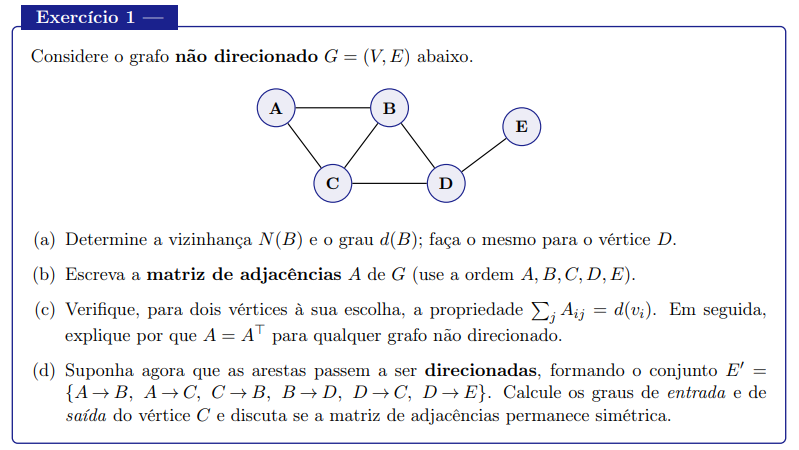
\includegraphics[width=0.7\textwidth]{imagens/ex1.png}
    \caption{Exercício 1.}
    \label{fig:ex1}
\end{figure}

\subsection{Letra a}
\[
N(B)=\{A,C,D\}
\]

\[
d(B)=|N(B)|=3
\]

\[
N(D)=\{B,C,E\}
\]

\[
d(D)=|N(D)|=3
\]
A vizinhança de um vértice é formada pelos vértices conectados diretamente a ele. Dessa forma, para o vértice \(B\), tem-se \(N(B)=\{A,C,D\}\), resultando em grau \(d(B)=3\). Analogamente, o vértice \(D\) possui como vizinhos \(B\), \(C\) e \(E\), de modo que \(N(D)=\{B,C,E\}\) e \(d(D)=3\).

\subsection{Letra b}
\[
\begin{array}{c|ccccc}
  & A & B & C & D & E \\ \hline
A & 0 & 1 & 1 & 0 & 0 \\
B & 1 & 0 & 1 & 1 & 0 \\
C & 1 & 1 & 0 & 1 & 0 \\
D & 0 & 1 & 1 & 0 & 1 \\
E & 0 & 0 & 0 & 1 & 0
\end{array}
\]

\subsection{Letra c}

Para o vértice $B$:

\[
\sum_j A_{Bj}
=
1+0+1+1+0
=
3
=
d(B).
\]

Para o vértice $D$:

\[
\sum_j A_{Dj}
=
0+1+1+0+1
=
3
=
d(D).
\]

Além disso, como o grafo é não direcionado,

\[
A_{ij}=A_{ji},
\]

logo,

\[
A=A^\top.
\]

Para verificar a propriedade \(\sum_j A_{ij}=d(v_i)\), foram escolhidos os vértices \(B\) e \(D\). Para \(B\), a soma dos elementos de sua linha na matriz de adjacências é \(1+0+1+1+0=3\), correspondendo ao seu grau \(d(B)=3\). Para \(D\), obtém-se \(0+1+1+0+1=3\), também correspondente a \(d(D)=3\). Além disso, por se tratar de um grafo não direcionado, sempre que existe uma aresta entre \(v_i\) e \(v_j\), existe adjacência tanto de \(v_i\) para \(v_j\) quanto de \(v_j\) para \(v_i\). Assim, \(A_{ij}=A_{ji}\), fazendo com que a matriz seja simétrica, isto é, \(A=A^\top\).

\subsection{Letra d}
As arestas que chegam ao vértice $C$ são:

\[
A\rightarrow C
\qquad \text{e} \qquad
D\rightarrow C.
\]

Portanto,

\[
d^{-}(C)=2.
\]

A única aresta que sai de $C$ é:

\[
C\rightarrow B.
\]

Assim,

\[
d^{+}(C)=1.
\]

Além disso,

\[
A\rightarrow B \in E',
\]

mas

\[
B\rightarrow A \notin E'.
\]

Logo,

\[
A_{AB}=1
\qquad \text{e} \qquad
A_{BA}=0,
\]

portanto,

\[
A\neq A^\top.
\]
Considerando o conjunto de arestas direcionadas \(E'\), chegam ao vértice \(C\) as arestas \(A\rightarrow C\) e \(D\rightarrow C\), resultando em grau de entrada \(d^-(C)=2\). A única aresta que parte de \(C\) é \(C\rightarrow B\), portanto seu grau de saída é \(d^+(C)=1\). Nesse caso, a matriz de adjacências deixa de ser necessariamente simétrica, pois uma aresta \(v_i\rightarrow v_j\) não implica a existência de \(v_j\rightarrow v_i\). Por exemplo, existe \(A\rightarrow B\), mas não \(B\rightarrow A\), de modo que \(A_{AB}=1\) e \(A_{BA}=0\). Assim, \(A\neq A^\top\).


\section{Exercício 2}

\begin{figure}[H]
    \centering
    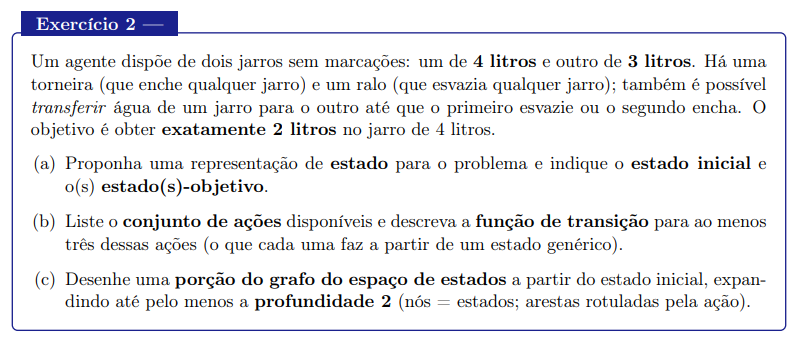
\includegraphics[width=0.7\textwidth]{imagens/ex2.png}
    \caption{Exercício 2.}
    \label{fig:ex2}
\end{figure}

\subsection{Letra a}
Define-se o estado como:

\[
(x,y),
\]

onde:

\[
0\leq x\leq4
\]

representa a quantidade de água no jarro de $4$ litros e

\[
0\leq y\leq3
\]

representa a quantidade de água no jarro de $3$ litros.

O estado inicial é:

\[
s_0=(0,0).
\]

Como o objetivo é obter exatamente $2$ litros no jarro de $4$ litros,
o conjunto de estados-objetivo é:

\[
G=\{(2,y)\mid 0\leq y\leq3\}.
\]

Explicitamente,

\[
G=\{(2,0),(2,1),(2,2),(2,3)\}.
\]
O estado do problema pode ser representado pelo par ordenado \((x,y)\), em que \(x\) corresponde à quantidade de água presente no jarro de 4 litros e \(y\) à quantidade presente no jarro de 3 litros. Dessa forma, \(0\leq x\leq4\) e \(0\leq y\leq3\). O estado inicial é \((0,0)\), pois ambos os jarros estão inicialmente vazios. Como o objetivo consiste em obter exatamente 2 litros no jarro de 4 litros, qualquer estado da forma \((2,y)\) é considerado objetivo.

\subsection{Letra b}
As ações possíveis são:

\[
\text{Encher}_{4}:(x,y)\rightarrow(4,y)
\]

\[
\text{Encher}_{3}:(x,y)\rightarrow(x,3)
\]

\[
\text{Esvaziar}_{4}:(x,y)\rightarrow(0,y)
\]

\[
\text{Esvaziar}_{3}:(x,y)\rightarrow(x,0)
\]

Para transferir água do jarro de $4$ litros para o de $3$ litros,
define-se:

\[
t=\min(x,3-y),
\]

resultando em:

\[
(x,y)\rightarrow(x-t,y+t).
\]

Para transferir água do jarro de $3$ litros para o de $4$ litros,
define-se:

\[
t=\min(y,4-x),
\]

resultando em:

\[
(x,y)\rightarrow(x+t,y-t).
\]
As ações disponíveis são: encher o jarro de 4 litros, encher o jarro de 3 litros, esvaziar o jarro de 4 litros, esvaziar o jarro de 3 litros, transferir água do jarro de 4 litros para o de 3 litros e realizar a transferência no sentido contrário. Nas ações de transferência, a operação continua até que o jarro de origem seja esvaziado ou que o jarro de destino atinja sua capacidade máxima. Por exemplo, na transferência do jarro de 4 litros para o de 3 litros, a quantidade transferida é \(t=\min(x,3-y)\), resultando no estado \((x-t,y+t)\).

\subsection{Letra c}
A partir do estado inicial:

\[
(0,0)
\]

são alcançados, na profundidade $1$:

\[
(4,0)
\qquad \text{e} \qquad
(0,3).
\]

Expandindo $(4,0)$:

\[
(4,0)\rightarrow(0,0)
\]

\[
(4,0)\rightarrow(4,3)
\]

\[
(4,0)\rightarrow(1,3).
\]

Expandindo $(0,3)$:

\[
(0,3)\rightarrow(0,0)
\]

\[
(0,3)\rightarrow(4,3)
\]

\[
(0,3)\rightarrow(3,0).
\]

Portanto:

\[
\begin{array}{c|l}
\text{Profundidade} & \text{Estados} \\ \hline
0 & (0,0) \\
1 & (4,0),(0,3) \\
2 & (0,0),(4,3),(1,3),(3,0)
\end{array}
\]

\begin{figure}[H]
\centering
\begin{tikzpicture}[
    >=Stealth,
    node distance=2.5cm and 3.5cm,
    estado/.style={
        draw,
        circle,
        minimum size=1.4cm,
        align=center
    },
    legenda/.style={
        align=center
    }
]

% Nós
\node[estado] (s0) at (0,0) {$(0,0)$};
\node[estado] (s1) at (-4,-2.5) {$(4,0)$};
\node[estado] (s2) at (4,-2.5) {$(0,3)$};
\node[estado] (s3) at (-7,-5) {$(1,3)$};
\node[estado] (s4) at (0,-5) {$(4,3)$};
\node[estado] (s5) at (7,-5) {$(3,0)$};

% Título superior
\node[legenda, above=0.8cm of s0] {\textbf{Estado inicial: ambos os jarros vazios}};

% Arestas do topo
\draw[->] (s0) -- node[above left, legenda] {Ação: encher jarro de 4 L} (s1);
\draw[->] (s0) -- node[above right, legenda] {Ação: encher jarro de 3 L} (s2);

% Arestas saindo de (4,0)
\draw[->] (s1) -- node[left, legenda] {Transferir do\\jarro de 4 L\\para o de 3 L} (s3);
\draw[->] (s1) -- node[above right, legenda] {Jarro\\de 3 L} (s4);

% Arestas saindo de (0,3)
\draw[->] (s2) -- node[above left, legenda] {Jarro\\de 4 L} (s4);
\draw[->] (s2) -- node[right, legenda] {Transferir do\\jarro de 3 L\\para o de 4 L} (s5);

% Observação embaixo do nó central
\node[legenda, below=0.8cm of s4] {Cheio: ambos os jarros cheios};

\end{tikzpicture}
\caption{Porção do grafo do espaço de estados do problema dos jarros até profundidade 2.}
\label{fig:grafo_jarros}
\end{figure}


\section{Exercício 3}

\begin{figure}[H]
    \centering
    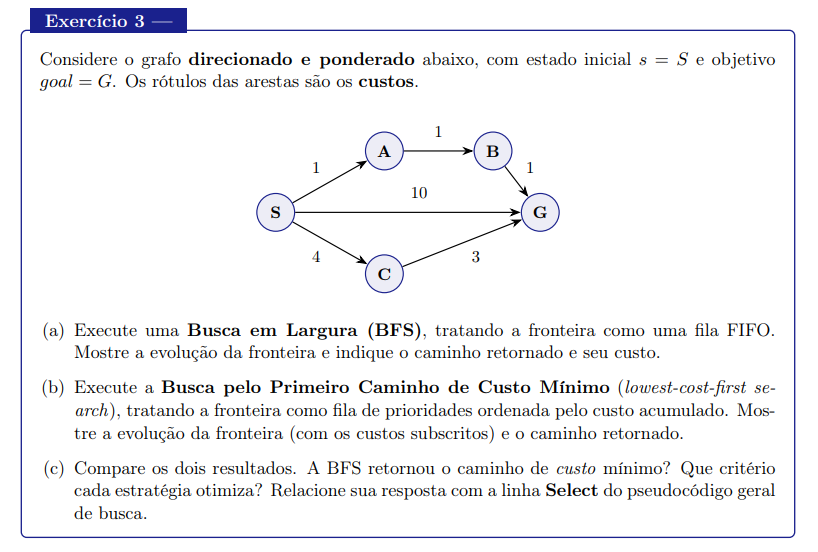
\includegraphics[width=0.7\textwidth]{imagens/ex3.png}
    \caption{Exercício 3.}
    \label{fig:ex3}
\end{figure}

\subsection{Letra a}
As arestas relevantes do grafo são:

\[
S \rightarrow A \;(1), \qquad
S \rightarrow C \;(4), \qquad
S \rightarrow G \;(10),
\]

\[
A \rightarrow B \;(1), \qquad
B \rightarrow G \;(1), \qquad
C \rightarrow G \;(3).
\]

A fronteira inicial é:

\[
F_0 = [\langle S\rangle_0].
\]

Expandindo $\langle S\rangle_0$:

\[
F_1 =
[
\langle S,A\rangle_1,
\langle S,C\rangle_4,
\langle S,G\rangle_{10}
].
\]

Seleciona-se $\langle S,A\rangle_1$ e expande-se $A$:

\[
F_2 =
[
\langle S,C\rangle_4,
\langle S,G\rangle_{10},
\langle S,A,B\rangle_2
].
\]

Seleciona-se $\langle S,C\rangle_4$ e expande-se $C$:

\[
F_3 =
[
\langle S,G\rangle_{10},
\langle S,A,B\rangle_2,
\langle S,C,G\rangle_7
].
\]

O próximo caminho selecionado é:

\[
\langle S,G\rangle_{10}.
\]

Como seu último vértice é o objetivo $G$, a busca termina.

Portanto,

\[
\boxed{\langle S,G\rangle_{10}}
\]

é o caminho retornado pela BFS.

\[
\begin{array}{c|l|l}
\text{Iteração} &
\text{Selecionado} &
\text{Fronteira após expansão} \\ \hline

0 &
\langle S\rangle_0 &
[\langle S,A\rangle_1,
 \langle S,C\rangle_4,
 \langle S,G\rangle_{10}] \\

1 &
\langle S,A\rangle_1 &
[\langle S,C\rangle_4,
 \langle S,G\rangle_{10},
 \langle S,A,B\rangle_2] \\

2 &
\langle S,C\rangle_4 &
[\langle S,G\rangle_{10},
 \langle S,A,B\rangle_2,
 \langle S,C,G\rangle_7] \\

3 &
\langle S,G\rangle_{10} &
\text{Objetivo encontrado}
\end{array}
\]
Na Busca em Largura, a fronteira é tratada como uma fila FIFO, de forma
que os caminhos de menor profundidade são considerados primeiro. O primeiro
caminho que alcança o objetivo é $\langle S,G\rangle_{10}$, portanto a BFS
retorna o caminho direto de $S$ até $G$, com custo total igual a $10$.

\subsection{Letra b}
A fronteira inicial é:

\[
F_0=[\langle S\rangle_0].
\]

Expandindo $S$, são obtidos:

\[
\langle S,A\rangle_1,
\qquad
\langle S,C\rangle_4,
\qquad
\langle S,G\rangle_{10}.
\]

Ordenando pelo custo acumulado:

\[
F_1=
[
\langle S,A\rangle_1,
\langle S,C\rangle_4,
\langle S,G\rangle_{10}
].
\]

O caminho de menor custo é $\langle S,A\rangle_1$.
Expandindo $A$:

\[
1+1=2,
\]

logo,

\[
\langle S,A,B\rangle_2.
\]

Assim,

\[
F_2=
[
\langle S,A,B\rangle_2,
\langle S,C\rangle_4,
\langle S,G\rangle_{10}
].
\]

Selecionando $\langle S,A,B\rangle_2$ e expandindo $B$:

\[
2+1=3,
\]

resultando em:

\[
\langle S,A,B,G\rangle_3.
\]

A fronteira passa a ser:

\[
F_3=
[
\langle S,A,B,G\rangle_3,
\langle S,C\rangle_4,
\langle S,G\rangle_{10}
].
\]

O caminho de menor custo é:

\[
\langle S,A,B,G\rangle_3.
\]

Como termina no objetivo $G$, a busca é encerrada.

Portanto,

\[
\boxed{\langle S,A,B,G\rangle_3}
\]

é o caminho retornado.

\[
\begin{array}{c|l|l}
\text{Iteração} &
\text{Selecionado} &
\text{Fronteira ordenada por custo} \\ \hline

0 &
\langle S\rangle_0 &
[\langle S,A\rangle_1,
 \langle S,C\rangle_4,
 \langle S,G\rangle_{10}] \\

1 &
\langle S,A\rangle_1 &
[\langle S,A,B\rangle_2,
 \langle S,C\rangle_4,
 \langle S,G\rangle_{10}] \\

2 &
\langle S,A,B\rangle_2 &
[\langle S,A,B,G\rangle_3,
 \langle S,C\rangle_4,
 \langle S,G\rangle_{10}] \\

3 &
\langle S,A,B,G\rangle_3 &
\text{Objetivo encontrado}
\end{array}
\]

Na Busca pelo Primeiro Caminho de Custo Mínimo, a fronteira é ordenada
pelo custo acumulado dos caminhos. Após as expansões, o primeiro caminho
até o objetivo selecionado é $\langle S,A,B,G\rangle_3$. Assim, o caminho
retornado é $S\rightarrow A\rightarrow B\rightarrow G$, com custo total
igual a $3$.

\subsection{Letra c}
Os caminhos retornados foram:

\[
\text{BFS: }
\langle S,G\rangle_{10}
\]

e

\[
\text{Custo mínimo: }
\langle S,A,B,G\rangle_3.
\]

Portanto,

\[
10 > 3.
\]

A BFS encontrou um caminho com apenas uma aresta:

\[
S\rightarrow G,
\]

enquanto a busca de custo mínimo encontrou:

\[
S\rightarrow A\rightarrow B\rightarrow G,
\]

com três arestas, porém menor custo total.

A BFS seleciona os caminhos segundo a profundidade:

\[
\operatorname{Select}_{\mathrm{BFS}}
=
\text{primeiro elemento da fila FIFO}.
\]

Já a Busca pelo Primeiro Caminho de Custo Mínimo seleciona:

\[
\operatorname{Select}_{\mathrm{LCF}}
=
\arg\min_{p\in F}\operatorname{cost}(p).
\]

\[
\begin{array}{c|c|c}
\text{Estratégia} &
\text{Caminho retornado} &
\text{Custo} \\ \hline

\text{BFS} &
\langle S,G\rangle &
10 \\

\text{Primeiro Caminho de Custo Mínimo} &
\langle S,A,B,G\rangle &
3
\end{array}
\]

A BFS não retornou o caminho de custo mínimo. Ela encontrou
$\langle S,G\rangle_{10}$, pois prioriza caminhos de menor profundidade,
ou seja, com menor número de arestas. Já a Busca pelo Primeiro Caminho de
Custo Mínimo retornou $\langle S,A,B,G\rangle_3$, pois seleciona sempre o
caminho de menor custo acumulado.

A diferença entre as estratégias está no critério utilizado pela operação
\textit{Select}: na BFS, seleciona-se o caminho mais antigo da fila FIFO;
na busca de custo mínimo, seleciona-se o caminho de menor custo acumulado.


\section{Exercício 4}

\begin{figure}[H]
    \centering
    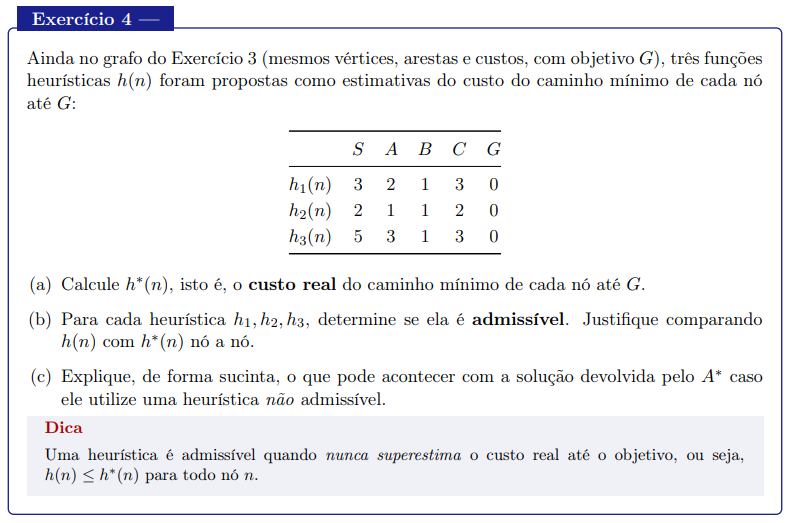
\includegraphics[width=0.7\textwidth]{imagens/ex4.png}
    \caption{Exercício 4.}
    \label{fig:ex4}
\end{figure}

\subsection{Letra a}
O valor $h^*(n)$ corresponde ao custo real do caminho mínimo
de cada vértice até o objetivo $G$.

Para o próprio objetivo:

\[
h^*(G)=0.
\]

Para $B$, existe a aresta direta

\[
B\rightarrow G,
\]

com custo $1$. Portanto,

\[
h^*(B)=1.
\]

Para $A$, o menor caminho até $G$ é

\[
A\rightarrow B\rightarrow G,
\]

logo,

\[
h^*(A)=1+1=2.
\]

Para $C$, o caminho até o objetivo é

\[
C\rightarrow G,
\]

com custo $3$. Assim,

\[
h^*(C)=3.
\]

Para $S$, existem três possibilidades:

\[
S\rightarrow G
\qquad\Rightarrow\qquad
10,
\]

\[
S\rightarrow C\rightarrow G
\qquad\Rightarrow\qquad
4+3=7,
\]

\[
S\rightarrow A\rightarrow B\rightarrow G
\qquad\Rightarrow\qquad
1+1+1=3.
\]

Portanto,

\[
h^*(S)=\min\{10,7,3\}=3.
\]

Assim,

\[
\boxed{
\begin{array}{c|ccccc}
n & S & A & B & C & G \\ \hline
h^*(n) & 3 & 2 & 1 & 3 & 0
\end{array}
}
\]

Os custos reais mínimos até o objetivo são obtidos analisando o menor
caminho de cada vértice até $G$. Dessa forma,

\[
h^*(S)=3,\qquad
h^*(A)=2,\qquad
h^*(B)=1,\qquad
h^*(C)=3,\qquad
h^*(G)=0.
\]

\subsection{Letra b}
Para $h_1$:

\[
\begin{array}{c|ccccc}
n & S & A & B & C & G \\ \hline
h_1(n) & 3 & 2 & 1 & 3 & 0 \\
h^*(n) & 3 & 2 & 1 & 3 & 0
\end{array}
\]

Verificando nó a nó:

\[
3\leq3,
\qquad
2\leq2,
\qquad
1\leq1,
\qquad
3\leq3,
\qquad
0\leq0.
\]

Logo,

\[
\boxed{h_1 \text{ é admissível}.}
\]

A heurística $h_1$ é admissível, pois seus valores coincidem com os
custos reais mínimos $h^*(n)$ para todos os vértices. Portanto,
$h_1(n)\leq h^*(n)$ em todos os casos.

Para $h_2$:

\[
\begin{array}{c|ccccc}
n & S & A & B & C & G \\ \hline
h_2(n) & 2 & 1 & 1 & 2 & 0 \\
h^*(n) & 3 & 2 & 1 & 3 & 0
\end{array}
\]

Verificando nó a nó:

\[
2\leq3,
\qquad
1\leq2,
\qquad
1\leq1,
\qquad
2\leq3,
\qquad
0\leq0.
\]

Logo,

\[
\boxed{h_2 \text{ é admissível}.}
\]

A heurística $h_2$ também é admissível, pois em nenhum vértice
ela superestima o custo real mínimo até $G$. Assim,
$h_2(n)\leq h^*(n)$ para todos os nós.

Para $h_3$:

\[
\begin{array}{c|ccccc}
n & S & A & B & C & G \\ \hline
h_3(n) & 5 & 3 & 1 & 3 & 0 \\
h^*(n) & 3 & 2 & 1 & 3 & 0
\end{array}
\]

Para $S$:

\[
h_3(S)=5>3=h^*(S).
\]

Para $A$:

\[
h_3(A)=3>2=h^*(A).
\]

Portanto, a condição

\[
h_3(n)\leq h^*(n)
\]

não é satisfeita para todos os nós.

Assim,

\[
\boxed{h_3 \text{ não é admissível}.}
\]

Para $h_3$:

\[
\begin{array}{c|ccccc}
n & S & A & B & C & G \\ \hline
h_3(n) & 5 & 3 & 1 & 3 & 0 \\
h^*(n) & 3 & 2 & 1 & 3 & 0
\end{array}
\]

Para $S$:

\[
h_3(S)=5>3=h^*(S).
\]

Para $A$:

\[
h_3(A)=3>2=h^*(A).
\]

Portanto, a condição

\[
h_3(n)\leq h^*(n)
\]

não é satisfeita para todos os nós.

Assim,

\[
\boxed{h_3 \text{ não é admissível}.}
\]

\[
\begin{array}{c|ccccc|c}
 & S & A & B & C & G & \text{Admissível?} \\ \hline
h^* & 3 & 2 & 1 & 3 & 0 & - \\
h_1 & 3 & 2 & 1 & 3 & 0 & \text{Sim} \\
h_2 & 2 & 1 & 1 & 2 & 0 & \text{Sim} \\
h_3 & 5 & 3 & 1 & 3 & 0 & \text{Não}
\end{array}
\]

\subsection{Letra c}
O algoritmo A* utiliza a função de avaliação

\[
f(n)=g(n)+h(n),
\]

em que $g(n)$ representa o custo acumulado até o nó $n$ e $h(n)$
representa uma estimativa do custo restante até o objetivo.

Se $h(n)$ não for admissível, pode ocorrer

\[
h(n)>h^*(n).
\]

Nesse caso, o custo estimado de um caminho pode ser maior do que seu
custo real, fazendo com que o A* priorize outro caminho.
Consequentemente, perde-se a garantia de obtenção da solução ótima.

Caso o A* utilize uma heurística não admissível, a estimativa pode
superestimar o custo real até o objetivo. Com isso, caminhos que poderiam
levar à solução ótima podem receber valores de avaliação maiores e serem
preteridos durante a busca. Portanto, o A* perde a garantia de retornar
uma solução de custo mínimo, podendo devolver uma solução subótima.

\section{Exercício 5}

\begin{figure}[H]
    \centering
    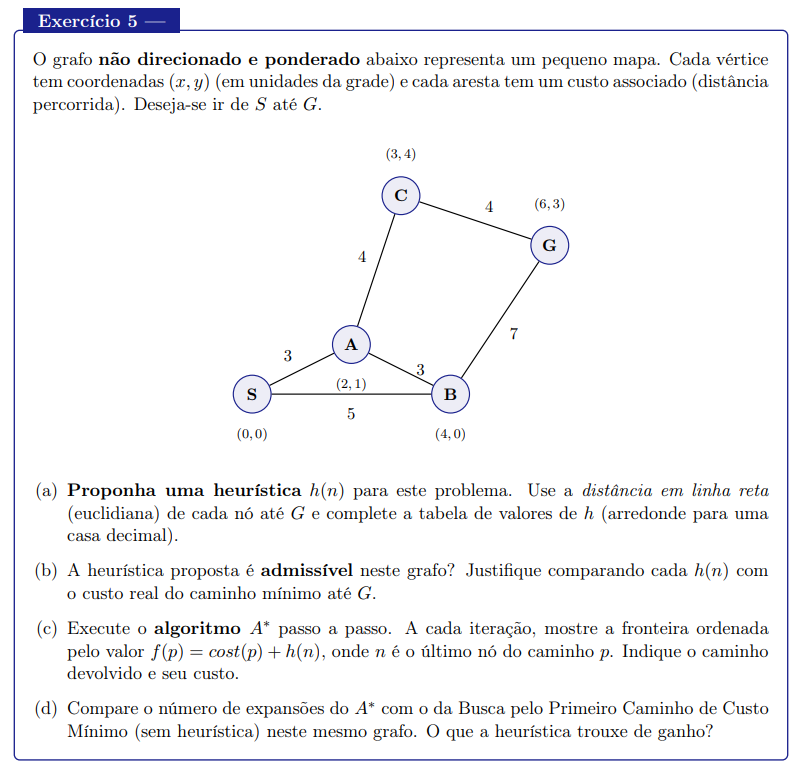
\includegraphics[width=0.7\textwidth]{imagens/ex5.png}
    \caption{Exercício 5.}
    \label{fig:ex5}
\end{figure}

\subsection{Letra a}
A heurística utilizada é a distância euclidiana entre cada vértice
$n=(x_n,y_n)$ e o objetivo $G=(6,3)$:

\[
h(n)=\sqrt{(x_n-6)^2+(y_n-3)^2}.
\]

Para $S=(0,0)$:

\[
h(S)=\sqrt{(0-6)^2+(0-3)^2}
=\sqrt{36+9}
=\sqrt{45}
\approx 6{,}7.
\]

Para $A=(2,1)$:

\[
h(A)=\sqrt{(2-6)^2+(1-3)^2}
=\sqrt{16+4}
=\sqrt{20}
\approx 4{,}5.
\]

Para $B=(4,0)$:

\[
h(B)=\sqrt{(4-6)^2+(0-3)^2}
=\sqrt{4+9}
=\sqrt{13}
\approx 3{,}6.
\]

Para $C=(3,4)$:

\[
h(C)=\sqrt{(3-6)^2+(4-3)^2}
=\sqrt{9+1}
=\sqrt{10}
\approx 3{,}2.
\]

Para o próprio objetivo:

\[
h(G)=0.
\]

Portanto,

\[
\boxed{
\begin{array}{c|ccccc}
n & S & A & B & C & G \\ \hline
h(n) & 6{,}7 & 4{,}5 & 3{,}6 & 3{,}2 & 0
\end{array}
}
\]

Adotou-se como heurística a distância euclidiana entre cada vértice e o
objetivo $G=(6,3)$. Os valores obtidos, arredondados para uma casa decimal,
foram:

\[
h(S)=6{,}7,\quad
h(A)=4{,}5,\quad
h(B)=3{,}6,\quad
h(C)=3{,}2,\quad
h(G)=0.
\]

\subsection{Letra b}
Para o objetivo:

\[
h^*(G)=0.
\]

Para $C$, o menor caminho é direto:

\[
C\rightarrow G,
\]

logo,

\[
h^*(C)=4.
\]

Para $B$, o menor caminho é:

\[
B\rightarrow G,
\]

portanto,

\[
h^*(B)=7.
\]

Para $A$, as principais possibilidades são:

\[
A\rightarrow C\rightarrow G:
\qquad 4+4=8,
\]

\[
A\rightarrow B\rightarrow G:
\qquad 3+7=10.
\]

Assim,

\[
h^*(A)=8.
\]

Para $S$:

\[
S\rightarrow A\rightarrow C\rightarrow G:
\qquad 3+4+4=11,
\]

\[
S\rightarrow B\rightarrow G:
\qquad 5+7=12,
\]

\[
S\rightarrow A\rightarrow B\rightarrow G:
\qquad 3+3+7=13.
\]

Logo,

\[
h^*(S)=11.
\]

Comparando os valores:

\[
\begin{array}{c|ccccc}
n & S & A & B & C & G \\ \hline
h(n)   & 6{,}7 & 4{,}5 & 3{,}6 & 3{,}2 & 0 \\
h^*(n) & 11    & 8     & 7     & 4     & 0
\end{array}
\]

Tem-se, nó a nó:

\[
6{,}7\leq11,
\qquad
4{,}5\leq8,
\qquad
3{,}6\leq7,
\qquad
3{,}2\leq4,
\qquad
0\leq0.
\]

Portanto,

\[
\boxed{h(n)\leq h^*(n)\;\; \forall n}
\]

e a heurística é admissível.

A heurística é admissível, pois em nenhum vértice a distância euclidiana
superestima o custo real do caminho mínimo até $G$. Para todos os nós,
verifica-se que

\[
h(n)\leq h^*(n).
\]

Assim, a heurística proposta satisfaz a condição de admissibilidade.

\subsection{Letra c}
O A* utiliza:

\[
f(p)=\operatorname{cost}(p)+h(n).
\]

Inicialmente:

\[
F_0=
[\langle S\rangle_0],
\]

com

\[
f(\langle S\rangle)=0+6{,}7=6{,}7.
\]

Expandindo $S$:

\[
\langle S,A\rangle_3:
\qquad
f=3+4{,}5=7{,}5,
\]

\[
\langle S,B\rangle_5:
\qquad
f=5+3{,}6=8{,}6.
\]

Logo,

\[
F_1=
[
\langle S,A\rangle_3\;(f=7{,}5),
\langle S,B\rangle_5\;(f=8{,}6)
].
\]

Seleciona-se $\langle S,A\rangle_3$.

A expansão de $A$ gera, entre os estados ainda relevantes:

\[
\langle S,A,B\rangle_6:
\qquad
f=6+3{,}6=9{,}6,
\]

\[
\langle S,A,C\rangle_7:
\qquad
f=7+3{,}2=10{,}2.
\]

Como já existe um caminho de menor custo para $B$,

\[
\langle S,B\rangle_5,
\]

o caminho $\langle S,A,B\rangle_6$ é descartado.

Assim,

\[
F_2=
[
\langle S,B\rangle_5\;(f=8{,}6),
\langle S,A,C\rangle_7\;(f=10{,}2)
].
\]

Seleciona-se $\langle S,B\rangle_5$.

Expandindo $B$, obtém-se:

\[
\langle S,B,G\rangle_{12},
\]

com

\[
f=12+h(G)=12.
\]

Logo,

\[
F_3=
[
\langle S,A,C\rangle_7\;(f=10{,}2),
\langle S,B,G\rangle_{12}\;(f=12)
].
\]

Seleciona-se $\langle S,A,C\rangle_7$.

Expandindo $C$:

\[
\langle S,A,C,G\rangle_{11},
\]

com

\[
f=11+h(G)=11.
\]

Como este caminho possui custo menor até $G$ que
$\langle S,B,G\rangle_{12}$, ele passa a ser a melhor opção.

Assim,

\[
F_4=
[
\langle S,A,C,G\rangle_{11}\;(f=11)
].
\]

O próximo caminho selecionado termina no objetivo $G$.
Portanto,

\[
\boxed{\langle S,A,C,G\rangle_{11}}
\]

é o caminho devolvido pelo A*.

\[
\begin{array}{c|l|l}
\text{Iteração}
&
\text{Selecionado}
&
\text{Fronteira ordenada por } f
\\ \hline

0 &
\langle S\rangle_0 &
[
\langle S,A\rangle_3\;(7{,}5),
\langle S,B\rangle_5\;(8{,}6)
]
\\

1 &
\langle S,A\rangle_3 &
[
\langle S,B\rangle_5\;(8{,}6),
\langle S,A,C\rangle_7\;(10{,}2)
]
\\

2 &
\langle S,B\rangle_5 &
[
\langle S,A,C\rangle_7\;(10{,}2),
\langle S,B,G\rangle_{12}\;(12)
]
\\

3 &
\langle S,A,C\rangle_7 &
[
\langle S,A,C,G\rangle_{11}\;(11)
]
\\

4 &
\langle S,A,C,G\rangle_{11} &
\text{Objetivo encontrado}
\end{array}
\]

Aplicando o algoritmo A*, a fronteira é ordenada de acordo com

\[
f(p)=\operatorname{cost}(p)+h(n).
\]

A sequência de vértices expandidos é $S$, $A$, $B$ e $C$. Após a expansão
de $C$, é obtido o caminho

\[
\langle S,A,C,G\rangle_{11},
\]

que passa a possuir o menor valor de $f$ na fronteira e termina no objetivo.
Portanto, o A* retorna o caminho

\[
\boxed{S\rightarrow A\rightarrow C\rightarrow G}
\]

com custo total igual a

\[
\boxed{11}.
\]

\subsection{Letra d}
Na Busca pelo Primeiro Caminho de Custo Mínimo, a seleção é realizada
apenas pelo custo acumulado.

Inicialmente:

\[
F_0=[\langle S\rangle_0].
\]

Expandindo $S$:

\[
F_1=
[
\langle S,A\rangle_3,
\langle S,B\rangle_5
].
\]

Seleciona-se $\langle S,A\rangle_3$.
A expansão produz um caminho para $C$ de custo $7$.
O caminho alternativo para $B$ possui custo $6$ e é pior que
$\langle S,B\rangle_5$.

Assim:

\[
F_2=
[
\langle S,B\rangle_5,
\langle S,A,C\rangle_7
].
\]

Selecionando $\langle S,B\rangle_5$:

\[
F_3=
[
\langle S,A,C\rangle_7,
\langle S,B,G\rangle_{12}
].
\]

Selecionando $\langle S,A,C\rangle_7$:

\[
F_4=
[
\langle S,A,C,G\rangle_{11}
].
\]

Em seguida, o objetivo é selecionado.

Portanto, a sequência de expansões é:

\[
S,\;A,\;B,\;C.
\]

O A* também expandiu:

\[
S,\;A,\;B,\;C.
\]

Logo,

\[
N_{\mathrm{A^*}}=4
\]

e

\[
N_{\mathrm{Custo\ minimo}}=4.
\]

Assim,

\[
\boxed{
N_{\mathrm{A^*}}
=
N_{\mathrm{Custo\ minimo}}
=
4
}
\]

Neste grafo, tanto o A* quanto a Busca pelo Primeiro Caminho de Custo
Mínimo expandem os vértices $S$, $A$, $B$ e $C$ antes de selecionar o
objetivo. Portanto, ambos realizam quatro expansões.

Assim, embora a heurística euclidiana seja admissível e forneça informação
sobre a proximidade do objetivo, neste exemplo específico ela não reduz o
número de expansões em relação à busca de custo mínimo. O pequeno tamanho e
a estrutura do grafo fazem com que as duas estratégias explorem os mesmos
vértices antes de alcançar a solução ótima.